\section{The \texttt{CASIER} solver}

\label{SectionCASIER}

\subsection{Introduction}

This section details the methodology used to represent the role of the floodplain with storage cells in the \texttt{MASCARET} system.

\vspace{0.5cm}

\texttt{MASCARET} allows to model the floodplain along a river by the mean of \textit{storage cells} or \textit{basins}, with the assumptions of uniform elevation water and zero speed. These storage cells are connected together and to the river by various exchange laws, function of the connection type. This allows to model a floodplain that does not actively contribute to the flow in the main channel. It is therefore an enhancement over channel-only 1D modelling, although it does not replace the accuracy of 2D modelling.

\vspace{0.5cm}

The following sections present the methodology used in \texttt{MASCARET}, the equations governing the various exchange flows through the links storage cell -- storage cell and river -- storage cell, the numerical coupling between the \texttt{CASIER} solver and the unsteady subcritical engine, the solution to the storage cell system and finally the vertical discretisation of the elevation/volume curve of the storage cell.

\vspace{0.5cm}

\subsection{General principle}

The system to be solved can be schematised as follows :

\begin{figure}[h]
    \begin{center}
     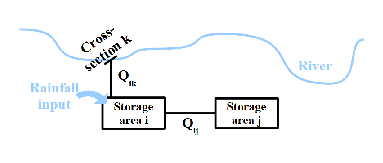
\includegraphics[scale=1.8]{Figures/CasierRiv.eps}
     \caption{Principle of Storage Cell -- River interaction}
    \end{center}
\end{figure}

The flow in the river is determined by solving the one dimensional Saint-Venant equations. In the \texttt{MASCARET} system, three computational engines can be used to solve the equations: a steady transcritical engine, an unsteady subcritical engine and an unsteady transcritical engine. This chapter only covers the coupling between the storage cell system and the unsteady subcritical engine. The algorithm used in the unsteady subcritical engine is a finite difference method with an implicit scheme, the details of which are given in section \ref{CplNyFlv}.

\vspace{0.5cm}

Regarding the storage cell system, the following assumptions are made :
\begin{itemize}
 \item the free surface elevation in each storage cell is \underline{horizontal};
 \item the flow speed in the storage cells is \underline{null};
 \item the discharge in the exchange links only depends on the free surface elevation in the storage cells and/or that in the river.
\end{itemize}

\vspace{0.5cm}

Each storage cell is therefore modelled by a continuity equation, which can be written at each time step $t$ :

\begin{equation}
 \label{EqCas}
 \frac{dV_{i}(Z_i)}{dt} = \sum_j Q_{ij} (Z_i,Z_j) + \sum_k Q_{ik} (Z_i,Z_k) + Q_{input,i}
\end{equation}

where :

\begin{itemize}
 \item $i$ and $j$ are indices for the storage cells;
 \item $k$ is the index for a computation section in a reach;
 \item $V_i$ is the volume of storage cell $i$;
 \item $Z_i$ is the free surface elevation in storage cell $i$, unknown;
 \item $Z_j$ is the free surface elevation in storage cell $j$, known at the previous time step;
 \item $Z_k$ is the river level elevation in the computation section $k$, as computed by the subcritical engine;
 \item $Q_{ij}$ is the discharge flowing from storage cell $j$ towards storage cell $i$, unknown;
 \item $Q_{ik}$ is the discharge flowing from the computation section $k$ in the river towards storage cell $i$, unknown;
 \item $Q_{input,i}$ is the discharge resulting from potential contributions (rain for example) in storage cell $i$, given by the user.
\end{itemize}

\vspace{0.5cm}

The water elevation in storage cell $i$ is therefore function of the exchange flows and potential input flows.

\vspace{0.5cm}

The exchange flows $Q_{ij}$ and $Q_{ik}$ are derived by solving the equations defining the exchange links (see section \ref{DebEch}).

\vspace{0.5cm}

The elevation $Z_k$ in the river is computed by the subcritical engine. The coupling between the storage cell system and the subcritical engine is described in section \ref{CplNyFlv}. The elevation in storage cell $i$ is then computed by solving the storage cell continuity equation, detailed in section \ref{ResContCas}.

\subsection{Derivation of the exchange flows}

\label{DebEch}

The exchange flow through the river - storage cell links, $Q_{ik}$, or storage cell - storage cell links, $Q_{ij}$, depends on the type of connection. The solver accepts four connection types : weir link, channel link, siphon link and orifice link.

\subsubsection{Weir link}

The discharge is computed from the weir formulation :

\begin{equation}
 Q = C m l \sqrt{2 g} h^{\frac{3}{2}}
\end{equation}

with :
\begin{itemize}
 \item $Q$ discharge in the link;
 \item $C$ correction coefficient (allows distinction between drowned or free flow);
 \item $m$ discharge coefficient;
 \item $l$ width of the weir;
 \item $h = Z_{u/s} - Z_{sill}$ the water depth above the weir ($Z_{u/s}$ is the elevation upstream of the weir, in the river or the storage cell, and $Z_{sill}$ is the elevation of the weir crest). The elevation upstream of the weir, $Z_{u/s}$, is provided by the flow engine.
\end{itemize}

\vspace{0.5cm}

It is therefore necessary to know the width of the weir, its elevation (representative average height) and its discharge coefficient.

\vspace{0.5cm}

It is good practice to calibrate only the discharge coefficient, the other parameters matching their associated real physical values.

\vspace{0.5cm}

\underline{Note} : the correction coefficient, $C$, makes it possible to represent the physics of the flow by taking account of the drowned or free flow conditions on the weir. It also allows to stabilise the numerical computation when the difference in elevation between the storage cells tends towards $0$. This is why it is called correction coefficient.



\subsubsection{Channel link}

The discharge is computed with the Manning-Strickler formulation, commonly used for free surface flows, with a check of the water depth upstream of the connection.

\vspace{0.5cm}

Two distinct cases are considered :

\begin{itemize}
 \item \textbf{Case 1} : case where the average bottom elevation of the channel is higher than the bottom elevation in the storage cells or the river (horizontal channel for example);
   \begin{figure}[h]
    \begin{center}
     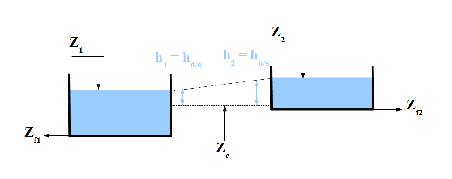
\includegraphics[scale=1.5]{Figures/Lchenal1.eps}
    \end{center}
   \end{figure}
   \vspace{0.5cm}
 \item \textbf{Case 2} : case where the average bottom elevation of the channel is lower than the bottom elevation in one of the storage cells (channel with uniform slope for example).
   \begin{figure}[h]
    \begin{center}
     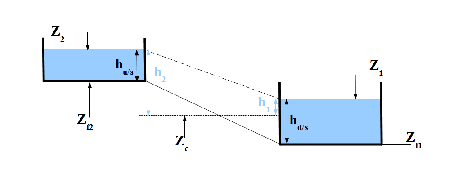
\includegraphics[scale=1.5]{Figures/Lchenal2.eps}
    \end{center}
   \end{figure}
\end{itemize}

\vspace{0.5cm}

where :
\begin{itemize}
 \item $Z_1$ and $Z_2$ are the free surface elevations in the storage cells or the river;
 \item $Z_{b1}$ and $Z_{b2}$ are the bottom elevations of the storage cells or the river;
 \item $Z_c$ is the average bottom elevation of the channel;
 \item $h_1$ and $h_2$ correspond to the water depths reduced to the average bottom elevation of the channel ($h_1 = Z_1 - Z_c$ and $h_2 = Z_2 - Z_c$). They allow to determine the direction of the flow and to distinguish upstream from downstream (index 2 refers to upstream);
 \item $h_{u/s}$ and $h_{d/s}$ correspond to the real water depths upstream and downstream of the connection. In case 1, they are computed relative to the average bottom elevation of the channel and are therefore equal to $h_1$ and $h_2$ respectively. In case 2, they are computed relative to the bottom elevations of the storage cells or the river ($h_{u/s} = Z_2 - Z_{b2}$ and $h_{d/s} = Z_1 - Z_{b1}$). It is necessary to calculate these values to test the presence of water upstream of the connection. If $h_{u/s} = 0$ (whereas $h_2 > 0$), the exchange flow will be null.
\end{itemize}

\vspace{0.5cm}

The exchange flow is function of $\Delta Z = |h_1 - h_2|$ and is calculated with the Manning-Strickler formula, commomn for free surface flows :

\begin{equation}
 Q = K S R_{h}^{\frac{2}{3}} \sqrt{\frac{\Delta Z}{L}}
\end{equation}
with :
\begin{itemize}
 \item $Q$ discharge in the link;
 \item $S$ wetted cross-section of the link;
 \item $R_h$ hydraulic radius of the link;
 \item $L$ length of the link;
 \item $K$ Strickler coefficient for the link ($m^{1/3}.s^{-1}$);
 \item $\Delta Z$ difference in elevation between the two storage cells or between the storage cell and the river.
\end{itemize}

\vspace{0.5cm}

The water depth in the channel $h$ is the average of $h_{u/s}$ and $h_{d/s}$. It is assumed that the water depth, $h$, is much smaller than the width, $l$, of the connection and that the hydraulic radius $R_h$ can be approximated by the water depth, in other words : $h \ll l$ and $R_h \simeq h$.

\vspace{0.5cm}

With these assumptions, the previous equation becomes :

\begin{equation}
 Q = K l h^{\frac{5}{3}} \sqrt{\frac{\Delta Z}{L}}
\end{equation}

\vspace{0.5cm}

However, when the elevation difference $\Delta Z$ tends towards $0$, this formulation is difficult to deal with, because the derivative of the flow relative to the difference in elevation then tends towards infinity. Numerically, this problem is addressed by introducing a correction coefficient $C$. This coefficient is automatically computed by the solver. The discharge then becomes :

\begin{equation}
 Q = C K l h^{\frac{5}{3}} \sqrt{\frac{\Delta Z}{L}}
\end{equation}

\vspace{0.5cm}

Therefore, to model this type of connection, it is necessary to know the average bottom elevation of the channel, its width, its length as well as its roughness coefficient. These parameters are supplied via the *.cas file or via the user interface.

\vspace{0.5cm}

It is good practice to try and calibrate only the roughness coefficient, the other parameters matching their associated real physical values.



\subsubsection{Siphon link}

The discharge is computed with the general equation for pressurised flows :

\begin{equation}
 Q = \sqrt{\frac{2 g}{\lambda L}\Delta Z} \times S^{\frac{5}{4}}
\end{equation}
with :
\begin{itemize}
 \item $Q$ discharge in the link;
 \item $S$ section of the siphon;
 \item $L$ length of the siphon;
 \item $\Delta Z$ the difference in elevation between the two storage cells or between the storage cell and the river, computed by the solver;
 \item $\lambda$ head loss coefficient with respect to the walls of the tunnel (from the Moody chart).
\end{itemize}

\vspace{0.5cm}

The siphon is considered pressurised when one of its extremities is covered with water. If the siphon is not pressurised (free surface flow), the siphon link is treated like a channel link, with the width calculated as the square root of the section $S$, and the Strickler coefficient calculated as :

\begin{equation}
 K = \sqrt{\frac{2 g}{\lambda} S^{\frac{1}{6}}}
\end{equation}

\vspace{0.5cm}

When the elevation difference $\Delta Z$ tends towards $0$, the discharge formulation above becomes unstable \cite{RISSOAN02}. As for the channel link, it is necessary to introduce a correction coefficient $C$. The flow formulation can then be rewritten :

\begin{equation}
 Q = C \sqrt{\frac{2 g}{\lambda L}\Delta Z} \times S^{\frac{5}{4}}
\end{equation}

\vspace{0.5cm}

Therefore, to model this type of connection, it is necessary to know the average bottom elevation of the siphon, its length and its section as well as the head loss coefficient, $\lambda$. These parameters are supplied via the *.cas file or via the user interface.

\vspace{0.5cm}

It is good practice to calibrate only the $\lambda$ coefficient, the other parameters matching their associated real physical values.



\subsubsection{Orifice link}

The figure below presents the methodology diagram for this type of connection :

\begin{figure}[h]
 \begin{center}
  \includegraphics[scale=1.]{Figures/Lorifice.eps}
 \end{center}
\end{figure}

where :
\begin{itemize}
 \item $Z_c$ is the invert level;
 \item $Z_p$ is the soffit level;
 \item $a=Z_p - Z_c$ is the height of the opening;
 \item $Z_{u/s}$ is the water elevation upstream of the connection, and $h_{u/s}$ the associated water depth : $h_{u/s} = Z_{u/s}-Z_c$;
 \item $Z_{d/s}$ is the water elevation downstream of the connection, and $h_{d/s}$ the associated water depth : $h_{d/s} = Z_{d/s}-Z_c$;
 \item $\epsilon$ is the contraction coefficient (along the vertical).
\end{itemize}

\vspace{0.5cm}

The connection is also defined by :
\begin{itemize}
 \item $B$ width of the opening;
 \item $S$ section of the opening : $S = a B$;
 \item $m$ discharge coefficient;
 \item The direction of flow:
   \begin{itemize}
     \item \underline{type 1} : the flow is possible in the 2 directions;
     \item \underline{type 2} : the flow is only possible in the direction upstream storage cell --> downstream storage cell or storage cell --> river;
     \item \underline{type 3} : the flow is only possible in the direction downstream storage cell --> upstream storage cell or river --> storage cell.
   \end{itemize}
\end{itemize}

\vspace{0.5cm}

The values for $Z_c$, $B$, $S$ and $m$ as well as the type of valve are specified by the user in the *.cas file or via the user interface. Parameters $a$ and $Z_p$ are calculated by the solver : $a = \frac{S}{B}$ and $Z_p = Z_c + a$.

\vspace{0.5cm}

The coefficient of vertical contraction, $\epsilon$, is calculated by the solver according to the height of the opening and the load ($h_{u/s}$) :

\begin{itemize}
 \item[*] if $0 \leq \frac{a}{h_{u/s}} < 0.55$ : $\epsilon = 0.65$;
 \item[*] if $0.55 \leq \frac{a}{h_{u/s}} < 0.9$ : $\epsilon = 0.5 + 0.268 \frac{a}{h_{u/s}}$;
 \item[*] if $0.9 \leq \frac{a}{h_{u/s}} \leq 1$ : $\epsilon = 0.745 + 0.255 \left ( \frac{a}{h_{u/s}} -0.9 \right )$.
\end{itemize}

\vspace{0.5cm}

The discharge calculation then depends on the type of flow :

\begin{itemize}
 \item \textbf{free surface flow} : $Z_{u/s} < Z_p$ \\
    The orifice behaves like a weir. The discharge is calculated as for the weir link, the modular limit $\alpha$ is set to 0.2 (see section \ref{CoefAct}). The elevation of the weir crest is taken equal to $Z_c$, its width to $B$. The discharge coefficient is taken from the *.cas file. The user must therefore specify two values for the discharge coefficient: one for a weir formulation and one for an orifice formulation;
 \item \textbf{drowned surcharged flow} : $Z_{u/s} > Z_p$ et $h_{d/s} > \frac{a}{2}$ \\
    The discharge is calculated using the following formulation :
    \begin{equation}
      Q = m \epsilon S \sqrt{2 g (h_{u/s}-h_{d/s})}
    \end{equation}
 \item \textbf{free surcharged flow} : $Z_{u/s} > Z_p$ et $h_{d/s} < \frac{a}{2}$ \\
    The discharge is computed using the following formulation :
    \begin{equation}
      Q = m \epsilon S \sqrt{2 g (h_{u/s}-\frac{a}{2})}
    \end{equation}
\end{itemize}

\vspace{0.5cm}

Finally, the calculation of the exchange flow velocity depends whether the orifice is surcharged or not :

\begin{itemize}
 \item \textbf{if the orifice is surcharged} :
   \begin{equation}
     V_{exch} = \frac{Q_{exch}}{S}
   \end{equation}
 \item \textbf{if the orifice is not surcharged} :
   \begin{equation}
     V_{exch} = \frac{Q_{exch}}{S_m}
   \end{equation}
   where $S_m = B . (Z_{avg}-Z_c)$ is the average wet surface above the connection. The average water level, $Z_{avg}$, is computed by the following formulations:
   \begin{itemize}
     \item if $Z_{d/s} < Z_c$ then $Z_{avg} = \frac{Z_{u/s}+Z_c}{2}$;
     \item if $Z_{d/s} > Z_c$ then $Z_{avg} = \frac{Z_{u/s}+Z_{d/s}}{2}$.
   \end{itemize}
\end{itemize}



\subsubsection{Drowning coefficient or correction coefficient}

\label{CoefAct}

\paragraph{Need for a correction coefficient\\}

\hspace*{1cm}

In the case of a weir link, when the flow becomes drowned, it is necessary to use the downstream elevation in the calculation of the discharge. The downstream elevation is introduced through the drowning coefficient, $C$.

\vspace{0.5cm}

Validation of the solver \cite{RISSOAN02} has shown that numerical instabilities occur, irrespective of the type of connection, when the difference in elevation between the storage cells or between a storage cell and the river tends towards 0. The drowning coefficient then also serves to stabilise the computation. This is why it is also called correction coefficient.

\vspace{0.5cm}

In the case of a weir link, the drowning coefficient is also used as correction coefficient. In the case of channel and siphon links, no drowning coefficient is required and a correction coefficient alone is applied.
The definition of the correction coefficient matches that used for the weir link.

\paragraph{Definition of the $C$ function\\}

\hspace*{1cm}

In the unsteady subcritical engine, drowned weirs are treated using a drowning coefficient, $C$, which is function of the variable, $R$ :

\begin{equation}
  R = \frac{Z_{d/s}-Z_{crest}}{Z_{u/s}-Z_{crest}}
\end{equation}

\vspace{0.5cm}

where $Z_{crest}$ is the elevation of the weir crest. Function $C$ has a parabolic shape; its derivative is not continuous around $1$. However, when solving the storage cells system, the derivative of the discharge appears explicitly in the computations \cite{GOUTAL_RISSOAN02}. It is therefore necessary that the $C$ function and its derivative are continuous.

\vspace{0.5cm}

On the other hand, the $C$ function depends on a parameter $\alpha$, which defines the activation period of the $C$ function. $C$ is thus defined only for : $R > \alpha$. In the case of a drowned weir link, the $\alpha$ coefficient corresponds to the drowned flow criteria.

The polynomial function $C(R,\alpha)$ has to satisfy the following conditions :

\begin{eqnarray}
  C(R=\alpha)=1 & \mbox{and} & C(R=1)=0 \nonumber \\
  \frac{dC}{dR}(R=\alpha)=0 & \mbox{and} & \frac{dC}{dR}(R=1)=0 \nonumber \\
  \frac{d^2 C}{dR^2}(R=\frac{1+\alpha}{2})=0
\end{eqnarray}

This results in a third order function instead of the parabolic function used in the subcritical engine for weirs in rivers. In addition to the continuity of its derivatives, this formulation yields a faster reduction of the discharge when the levels of the two connected storage cells become closer.

\vspace{0.5cm}

The selected function is defined as follows :
\begin{itemize}
 \item in free flow mode and without correction : $R<\alpha$ and $C=1$;
 \item in drowned mode and/or with correction : $R>=\alpha$ ($R<1$ in all the cases) and :
   \begin{equation}
     C = -2 \left ( \frac{1-R}{1-\alpha} \right )^3 + 3 \left ( \frac{1-R}{1-\alpha} \right )^2
   \end{equation}
\end{itemize}

\vspace{0.5cm}

The $\alpha$ parameter is set to 0.95 for the channel and siphon links and varies between 0.2 and 0.8 for the weir links. It is set by the user according to the type of weir.

\vspace{0.5cm}

The variable $R$ is calculated relative to the $Z_{crest}$ elevation, which corresponds to the elevation of the weir crest, or to the average bottom level of the channel or that of the siphon.

\begin{figure}
  \begin{center}
    \includegraphics[scale=0.5,angle=270]{Figures/CR.eps}
    \caption{Function $C=f(R)$}
  \end{center}
\end{figure}



\subsubsection{Contribution of rain}

The user specifies the flows due to rainfall through the definition of a hydrograph $Q(t)$. The discharge at time $t$ is taken as an average of the provided discharges at times $t$ and $t - dt$. The interpolation of the flows from the hydrograph is linear.



\subsection{Coupling with the subcritical engine}

\label{CplNyFlv}

The storage cells and the river are implicitly coupled with the help of a state-transition matrix \ref{eq1}. Two new equations are introduced to reflect :
\vspace{0.5cm}

\begin{itemize}
 \item the exchange flow in the links;
   \begin{equation}
     A_{link}\Delta Q_{link}+B_{link}\Delta Z_{u/s} + C_{link}\Delta Z_{d/s} = D_{link}
   \end{equation}
   \vspace{0.5cm}
 \item and the change of the water level in the storage cells;
    \begin{equation}
     S_{cell}\frac{\Delta Z_{cell}}{\Delta t} = \Sigma Q_{link}
   \end{equation}
\end{itemize}

\vspace{0.5cm}

where $S_{cell}$ is the surface of a storage cell and :

\begin{equation*}
 A_{link} = -1 \mbox{ ; } B_{link} = \frac{\partial Q}{\partial Z_{u/s}} \mbox{ ; }  C_{link} = \frac{\partial Q}{\partial Z_{d/s}} \mbox{ ; } D_{link} = 0
\end{equation*}


\vspace{0.5cm}

For each storage cell anf each connection, the size of system \ref{eq1} is increased with one variable and one equation. In the case of a river - storage cell link, the shallow water equations on the corresponding river cross-sections are replaced.
The continuity equation becomes an equality between the flow discharges and the momentum equation is an equality between the water levels.

\vspace{0.5cm}

For the simple case of a reach with only 7 cross-sections, the initial shallow water system of equations is :

\begin{equation}
    \left(
         \begin{array}{cccccccccccc}
          \scriptscriptstyle -J & \scriptscriptstyle G & \scriptscriptstyle H & & & & & & & & & \\
           \scriptscriptstyle -O & \scriptscriptstyle L & \scriptscriptstyle M & & & & & & & & & \\
              & \scriptscriptstyle -I & \scriptscriptstyle -J & \scriptscriptstyle G & \scriptscriptstyle H & & & & & & & \\
              & \scriptscriptstyle -N & \scriptscriptstyle -O & \scriptscriptstyle L & \scriptscriptstyle M & & & &  & & & \\
              & & & \scriptscriptstyle -I & \scriptscriptstyle -J & \scriptscriptstyle G & \scriptscriptstyle H & & & & & \\
              & & & \scriptscriptstyle -N & \scriptscriptstyle -O & \scriptscriptstyle L & \scriptscriptstyle M & & & & & \\
              & & & & & \scriptscriptstyle -I & \scriptscriptstyle -J & \scriptscriptstyle G & \scriptscriptstyle H & & & \\
              & & & & & \scriptscriptstyle -N & \scriptscriptstyle -O & \scriptscriptstyle L & \scriptscriptstyle M & & & \\
              & & & & & & & \scriptscriptstyle -I & \scriptscriptstyle -J & \scriptscriptstyle G & \scriptscriptstyle H & \\
              & & & & & & & \scriptscriptstyle -N & \scriptscriptstyle -O & \scriptscriptstyle L & \scriptscriptstyle M & \\
              & & & & & & & & & \scriptscriptstyle -I & \scriptscriptstyle -J & \scriptscriptstyle G \\
              & & & & & & & & & \scriptscriptstyle -N & \scriptscriptstyle -O & \scriptscriptstyle L \\
         \end{array}
    \right)
    \left(
            \begin{array}{c}
               \scriptscriptstyle \Delta Z_1\\
               \scriptscriptstyle \Delta Q_2\\
               \scriptscriptstyle \Delta Z_2\\
               \scriptscriptstyle \Delta Q_3\\
               \scriptscriptstyle \Delta Z_3\\
               \scriptscriptstyle \Delta Q_4\\
               \scriptscriptstyle \Delta Z_4\\
               \scriptscriptstyle \Delta Q_5\\
               \scriptscriptstyle \Delta Z_5\\
               \scriptscriptstyle \Delta Q_6\\
               \scriptscriptstyle \Delta Z_6\\
               \scriptscriptstyle \Delta Q_7
            \end{array}
    \right)
     =
    \left(
            \begin{array}{c}
               \scriptscriptstyle K\\
               \scriptscriptstyle P\\
               \scriptscriptstyle K\\
               \scriptscriptstyle P\\
               \scriptscriptstyle K\\
               \scriptscriptstyle P\\
               \scriptscriptstyle K\\
               \scriptscriptstyle P\\
               \scriptscriptstyle K\\
               \scriptscriptstyle P\\
               \scriptscriptstyle K\\
               \scriptscriptstyle P
            \end{array}
    \right)
\end{equation}

\vspace{0.5cm}

A storage cell with a link in between the river cross-sections $4$ and $5$ gives the following system :

\begin{equation}
    \left(
         \begin{array}{cccccccccccccc}
          \scriptscriptstyle -J & \scriptscriptstyle G & \scriptscriptstyle H & & & & & & & & & & &\\
           \scriptscriptstyle -O & \scriptscriptstyle L & \scriptscriptstyle M & & & & & & & & &  & &\\
              & \scriptscriptstyle -I & \scriptscriptstyle -J & \scriptscriptstyle G & \scriptscriptstyle H & & & & & & &  & &\\
              & \scriptscriptstyle -N & \scriptscriptstyle -O & \scriptscriptstyle L & \scriptscriptstyle M & & & &  & & &  & &\\
              & & & \scriptscriptstyle -I & \scriptscriptstyle -J & \scriptscriptstyle G & \scriptscriptstyle H & & & & &  & &\\
              & & & \scriptscriptstyle -N & \scriptscriptstyle -O & \scriptscriptstyle L & \scriptscriptstyle M & & & & &  & &\\
              & & & & & \scriptscriptstyle 1 & & \scriptscriptstyle -1 & & & &  & &\\
              & & & & & & \scriptscriptstyle 1 & & \scriptscriptstyle -1 & & &  & &\\
              & & & & & & & \scriptscriptstyle -I & \scriptscriptstyle -J & \scriptscriptstyle G & \scriptscriptstyle H &  & &\\
              & & & & & & & \scriptscriptstyle -N & \scriptscriptstyle -O & \scriptscriptstyle L & \scriptscriptstyle M &  & &\\
              & & & & & & & & & \scriptscriptstyle -I & \scriptscriptstyle -J & \scriptscriptstyle G  & &\\
              & & & & & & & & & \scriptscriptstyle -N & \scriptscriptstyle -O & \scriptscriptstyle L  & &\\
              & & & & & & \scriptscriptstyle B & & \scriptscriptstyle C & & & & \scriptscriptstyle A &\\
              & & & & & & & & & & & &  \scriptscriptstyle -1 & \scriptscriptstyle \frac{S}{\Delta t}\\
         \end{array}
    \right)
    \left(
            \begin{array}{c}
               \scriptscriptstyle \Delta Z_1\\
               \scriptscriptstyle \Delta Q_2\\
               \scriptscriptstyle \Delta Z_2\\
               \scriptscriptstyle \Delta Q_3\\
               \scriptscriptstyle \Delta Z_3\\
               \scriptscriptstyle \Delta Q_4\\
               \scriptscriptstyle \Delta Z_4\\
               \scriptscriptstyle \Delta Q_5\\
               \scriptscriptstyle \Delta Z_5\\
               \scriptscriptstyle \Delta Q_6\\
               \scriptscriptstyle \Delta Z_6\\
               \scriptscriptstyle \Delta Q_7 \\
               \scriptscriptstyle \Delta Q_l \\
               \scriptscriptstyle \Delta Z_c
            \end{array}
    \right)
     =
    \left(
            \begin{array}{c}
               \scriptscriptstyle K\\
               \scriptscriptstyle P\\
               \scriptscriptstyle K\\
               \scriptscriptstyle P\\
               \scriptscriptstyle K\\
               \scriptscriptstyle P\\
               \scriptscriptstyle \Sigma Q\\
               \scriptscriptstyle \Sigma Z\\
               \scriptscriptstyle K\\
               \scriptscriptstyle P\\
               \scriptscriptstyle K\\
               \scriptscriptstyle P \\
               \scriptscriptstyle D \\
               \scriptscriptstyle Q_l
            \end{array}
    \right)
\end{equation}

\vspace{0.5cm}


\subsection{Data pre-processing}

The engine for the storage cell system requires that the area at the free surface $S(Z)$ and the associated volume $V(Z)$ are known for each free surface elevation $Z$ in a storage cell. It is therefore necessary to define the laws $S(Z)$ and $V(Z)$, which link an area and a volume to a given elevation. These laws need to be discretised, they are not continuous functions. They have a well-defined number of pairs $(S,Z)$ and $(V,Z)$ and the increment between elevations is constant (vertical discretisation). 
%The increment between the elevations is called vertical discretisation step.

\vspace{0.5cm}

The user can enter these discretised laws $S(Z)$ and $V(Z)$ \textit{manually}, i.e. by editing directly the file holding the storage cell geometry. However, these laws are often difficult to determine. Here the user can ask that they are computed automatically by the solver, after having defined the border points and the interior points characteristic of the storage cell.

\vspace{0.5cm}

The principle of automatic vertical discretisation is as follows.

\vspace{0.5cm}

$\Longrightarrow$ \textbf{Computation of the elevations}

\vspace{0.5cm}

The elevations of the interior points are sorted in ascending order in an array called $Z_{INT}$.

\vspace{0.5cm}

By definition $Z_{INT}$ is such that :

$Z_{INT}(i-1) <= Z_{INT}(i)$ for $i=2..$ number of interior points.

\vspace{0.5cm}

$Z$ is the array containing the discretised elevations.

\vspace{0.5cm}

The first discretised elevation is the lowest elevation from the interior points : \\
$Z(1) = Min(Z(i),\mbox{ }i=1..\mbox{number of interior points}) = Z_{INT}(1)$.

\vspace{0.5cm}

The elevations are then sorted in ascending order with : \\
$Z(i+1)-Z(i) = $ vertical discretisation step.

\vspace{0.5cm}

The number of elevations is equal to the chosen number of vertical discretisation steps $N_{planim}$.

\vspace{0.5cm}

The topmost elevation is defined as follows :
 \begin{eqnarray}
 Z(N_{planim}) & = & Z(1) \nonumber \\
                & + & (N_{planim}-1) \nonumber \\
                & \times & \mbox{vertical discretisation step} \nonumber
 \end{eqnarray}

\vspace{0.5cm}

$\Longrightarrow$ \textbf{Computation of the areas}

\vspace{0.5cm}

The border points define the maximum area of the storage cell ($S_{max}$) : this area is computed from the definition of the area of a polygon. If the user has chosen the computation option whereby the area can be defined independently of the elevation, the area of the storage cell is equal to $S_{max}$ irrespective of the elevation in the storage cell.

\vspace{0.5cm}

Otherwise, the first area is computed as follows :

\vspace{0.5cm}

$S(1) = S_{max} \times$ (number of interior points with reference elevation $Z(1)$) / (number of interior points)

\vspace{0.5cm}

If $Z_{max}$ is the highest elevation from the interior points :

\begin{eqnarray}
Z_{max} & = & Max(Z(i),\mbox{ }i = 1..\mbox{number of interior points}) \nonumber \\
        & = & Z_{INT}(\mbox{number of interior points}) \nonumber
\end{eqnarray}

\vspace{0.5cm}

As long as this elevation is not reached, $S(i)$ is computed as follows :

\vspace{0.5cm}

given $k$ such that : $Z_{int}(k-1) \leq Z(i) < Z_{INT}(k)$

\begin{equation}
  S_1 = \frac{k-1}{\mbox{size}(Z_{INT})}S_{max}
\end{equation}

where $\mbox{size}(Z_{INT})$ is the size of array $Z_{INT}$.

\begin{equation}
  S_2 = \frac{k}{\mbox{size}(Z_{INT})}S_{max}
\end{equation}

\begin{equation}
  \alpha = \frac{Z(i)-Z_{INT}(k-1)}{Z_{INT}(k)-Z_{INT}(k-1)}
\end{equation}

\begin{equation}
  S(i) = (1-\alpha) \times S_1 + \alpha \times S_2
\end{equation}

\vspace{0.5cm}

When $Z_{max}$ is reached or exceeded, the area is equal to the maximum area of the storage cell : $S(i) = S_{max}$.

\vspace{0.5cm}

$\Longrightarrow$ \textbf{Computation of the volumes}

\vspace{0.5cm}

With regard to volumes, the first volume is null : $V(1) = 0$ since it is associated to the bottom elevation of the storage cell, i.e. the storage cell is empty.
The other volumes are defined by the relationship :

\vspace{0.5cm}

$V(i) = V(i-1) + [(S(i-1) + S(i)) / 2] \times$ vertical discretisation step

\begin{landscape}

\begin{table}
\centering  
\caption{Summary table of the laws S(Z) and V(Z)}
\vspace{0.25cm}
\begin{tabular}{c|c|c}
  \textbf{Elevation, Z} &\textbf{Area, S} & \textbf{Volume, V} \\
  \hline
  \multirow{5}{*}{$Z(1) = Z_{INT}(1)$} & $S(1) = S_{max} \times$ & \multirow{5}{*}{$V(1)=0$} \\
                                       & \footnotesize{(number of interior} & \\
                                       & \footnotesize{points with reference} & \\
                                       & \footnotesize{elevation } $Z(1)$) / & \\
                                       & \footnotesize{(number of interior points)} & \\
  \hline
  $Z(i)=Z(i-1)+$ & $S(i)=S(i-1)+\Delta S$ & $V(i)=V(i-1)+$  \\
  \footnotesize{vertical discretisation step}   & $\Delta S = (1-\alpha)S_1 + \alpha S_2$ & $(S(i-1)+S(i))/2 \times$ \\
                                       &                                         & \footnotesize{vertical discretisation step} \\
  \hline
  $Z(i)\geq Z_{INT}$ \footnotesize{(number of} & \multirow{3}{*}{$S(i) = S_{max}$} & $V(i)=V(i-1)+$  \\
  \footnotesize{interior points)}            &                  &  $(S(i-1)+S(i))/2 \times$ \\
                                               &                  & \footnotesize{vertical discretisation step} \\
  \hline
  $Z$ \footnotesize{(number of steps} & $S$ \footnotesize{(number of steps} & $V(i)=V(i-1)+$  \\
  \footnotesize{of vertical discretisation)} $=Z(1)$ & \footnotesize{of vertical discretisation)} $=S_{max}$ & $(S(i-1)+S(i))/2 \times$ \\
  $+$ \footnotesize{(number of steps of} &                   & \footnotesize{vertical discretisation steps} \\
  \footnotesize{vertical discretisation }$-1$\footnotesize{)} $\times$ & & \\
  \footnotesize{vertical discretisation step} & & \\
  \hline
 \end{tabular}
\end{table}

\end{landscape}

\textsc{\textbf{Example}} :

\vspace{0.25cm}

In this example, figure \ref{PlanimCasier}) shows an plan view of a storage cell and identifies the location of the interior points with associated elevations. The points are located by their coordinates $(X,Y)$.

\begin{figure}
    \begin{center}
     \includegraphics[scale=0.4,angle=270]{Figures/PlanimCasier.eps}
     \vspace{1.cm}
     \caption{Example of vertical discretisation of a storage cell}
     \label{PlanimCasier}
    \end{center}
\end{figure}

The vertical discretisation step is 1 m, the number of vertical discretisation steps is 10.

\vspace{0.5cm}

In this example, the solver determines the laws $S(Z)$ and $V(Z)$ indicated in table \ref{ExPlan}.

\begin{table}
  \centering  
  \caption{Example of vertical discretisation result}
  \label{ExPlan}
  \vspace{0.25cm}
  \begin{tabular}{c|c|c}
  \textbf{Elevation, Z $(m)$} &\textbf{Area, S $(m^2)$} & \textbf{Volume, V $(m^3)$} \\
 \hline
  2 & 22.5 & 0 \\
  3 & 33.8 & 28.1 \\
  4 & 67.5 & 78.8 \\
  5 & 78.8 & 151.9 \\
  6 & 90 & 236.3 \\
  7 & 90 & 326.3 \\
  8 & 90 & 416.3 \\
  9 & 90 & 506.3 \\
 10 & 90 & 596.3 \\
 11 & 90 & 686.3 \\
  \hline
  \end{tabular}
\end{table}

